\subsection{Durchführung des Großtests 2}

Nach dem letzten Test wurde der Code so erweitert, dass Bluetooth nur
noch 4 Verbindungen gleichzeitig aufbaut und in regelmäßigen Abständen
alte Verbindungen fallen lässt. Das hindert den Bluetooth Adapter zu
schnell zu überlasten.

Außerdem wurden weitere Kommilitonen darum gebeten am Test teilzunehmen.
Insgesamt wurde der Test von 9 Personen mit 14 Handys ausgeführt.

Die Benennung der Handys wurde den einzelnen Personen überlassen. Es
wurde dafür gesorgt, dass alle Handys den Kontakt der anderen Handys
kennen.


\subsubsection{Ergebnisse Test 1}

Wir haben auf 167 Nachrichten 8 erfolgreiche Fälle und 159 Errors.

\paragraph{Folgende Beispiele veranschaulichen Nachrichten, die beim
Empfänger angekommen sind:}

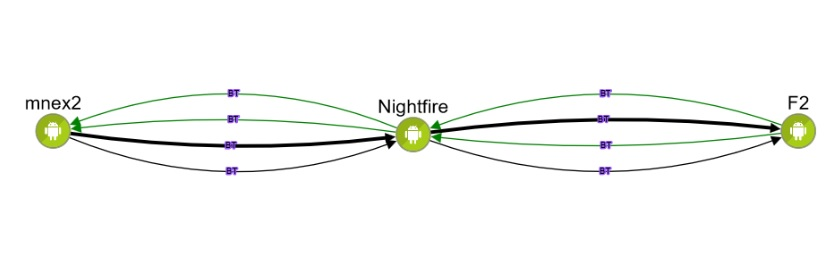
\includegraphics[width=1.0\textwidth]{belege/grosstests/Bilder/Grosstest2/Test1Erfolg2.jpg}
1. mnex2 sendet eine Nachricht an F2. Diese kommt erst nach einer
Retransmission an. Das Acknowledgement kommt auch erst beim 2. Versuch
an.

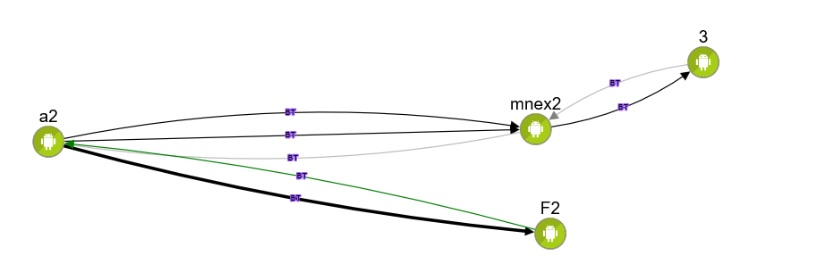
\includegraphics[width=1.0\textwidth]{belege/grosstests/Bilder/Grosstest2/Test1Erfolg1.jpg}

2. Hier sendet a2 eine Nachricht an F2. Da F2 ein Nachbar ist, kommt die
Nachricht direkt an. A2 versucht gleichzeitig auch noch einen weiteren
Weg, der jedoch nach einem Hop verloren geht.

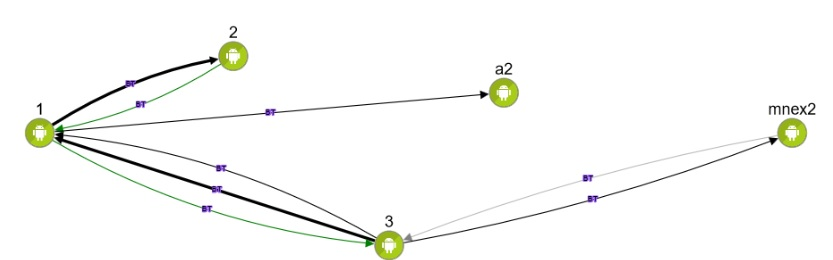
\includegraphics[width=1.0\textwidth]{belege/grosstests/Bilder/Grosstest2/Test1Erfolg3.jpg}

3. In dieser Nachricht sendet 3 an 2. Die Nachricht wird erfolgreich über 1
geschickt. 1 sendet die Nachricht gleichzeitig auch noch an a2.

\paragraph{Folgende Beispiele veranschaulichen Nachrichten, die nicht beim
Empfänger angekommen sind:}

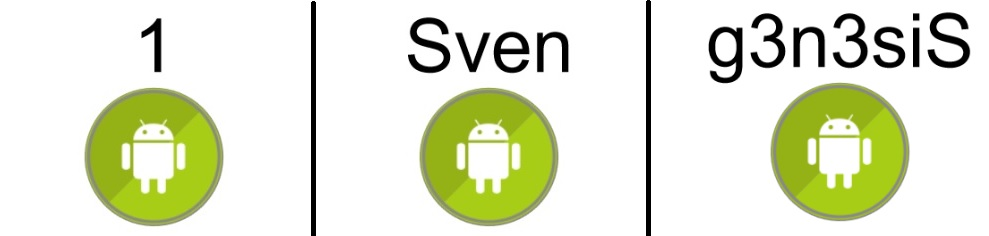
\includegraphics[width=1.0\textwidth]{belege/grosstests/Bilder/Grosstest2/Test1Misserfolg2.jpg}

1. Bei diesem Test kam es häufig zur Situation, dass Handys überhaupt keine
Verbindung mit anderen Geräten herstellen konnten. Dies kann daran
liegen, dass die Geräte in der näheren Umgebung bereits 4 Verbindungen
offen hatten, oder dessen Bluetooth durch frühere Transmissions
überlastet war.

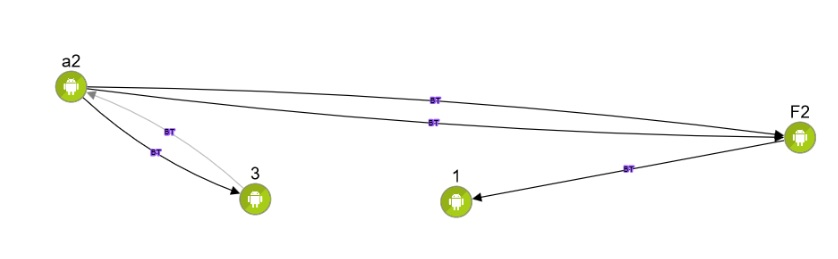
\includegraphics[width=1.0\textwidth]{belege/grosstests/Bilder/Grosstest2/Test1Misserfolg1.jpg}

2. Hier sendet a2 eine Nachricht, die jedoch nur über einen Hop
weitergeleitet wird und deshalb nicht ankommt.

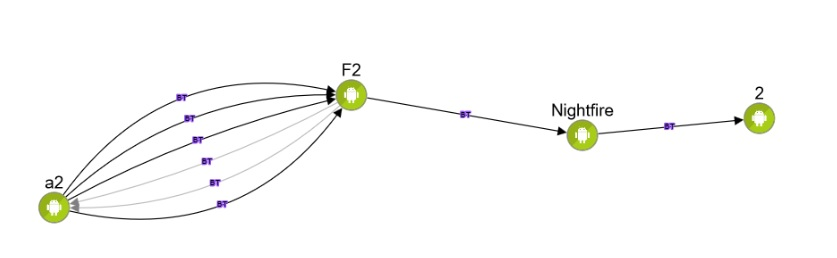
\includegraphics[width=1.0\textwidth]{belege/grosstests/Bilder/Grosstest2/Test1Misserfolg3.jpg}

3. Auch hier sendet a2 eine Nachricht, die über die Hops F2, Nightfire und
2 läuft, dort jedoch verloren geht.

\paragraph{Schlussfolgerung aus dem Test:}

Die Einschränkung auf 4 Verbindungen pro Bluetooth-Gerät scheint nicht
erfolgreich gewesen zu sein. Der Bluetoothadapter scheint immer noch
sehr schnell zu überlasten. Die Einschränkung führt außerdem noch dazu,
dass nicht alle Handys in der Umgebung erreicht werden, da bereits 4
Verbindungen bestehen, oder versucht aufgebaut zu werden.\\

Es bestand kein Grund zur Annahme, dass Verbindungen bei diesem Test
nicht zustande gekommen sind, weil ein Handy in den Standby-Modus
gegangen ist.


\subsubsection{Ergebnisse Test 2}

Wir haben auf 227 Nachrichten 20 erfolgreiche Fälle und 7 Errors.

\paragraph{Folgende Beispiele veranschaulichen Nachrichten, die beim Empfänger angekommen sind:}

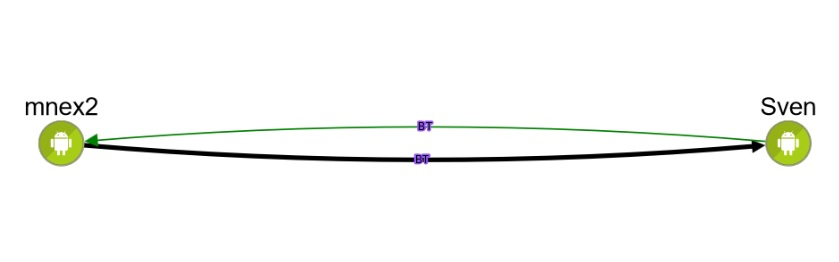
\includegraphics[width=1.0\textwidth]{belege/grosstests/Bilder/Grosstest2/Test2Erfolg1.jpg}

1. Die Verbindung zwischen mnex2 und Sven bestand über den ganzen Test.
Über diese Verbindung gingen 13 Nachrichten.

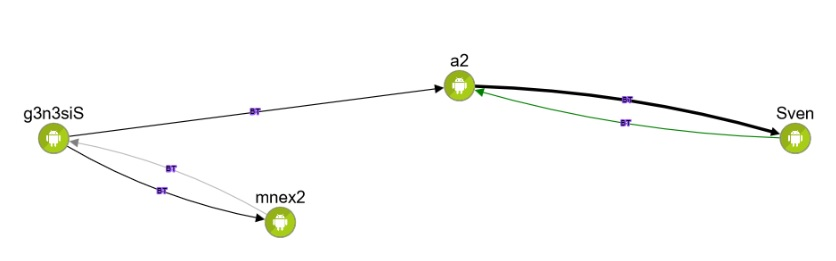
\includegraphics[width=1.0\textwidth]{belege/grosstests/Bilder/Grosstest2/Test2Erfolg3.jpg}

2. G3n3siS sendet eine Nachricht an Sven. Diese wird erfolgreich an a2
übermittelt, welches diese dann an Sven weiterleitet. Das
Acknowledgement kommt jedoch nicht mehr zurück.

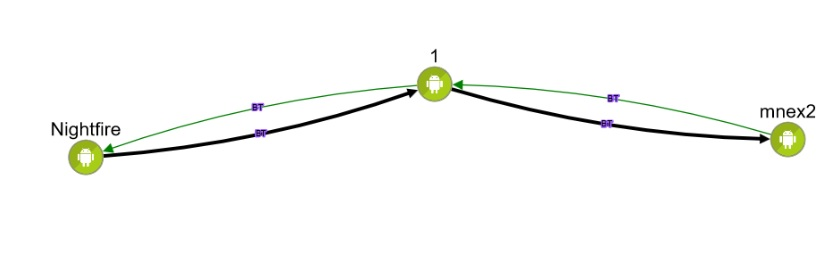
\includegraphics[width=1.0\textwidth]{belege/grosstests/Bilder/Grosstest2/Test2Erfolg4.jpg}

3. Nightfire sendet eine Nachricht an mnex2.

\paragraph{Folgende Beispiele veranschaulichen Nachrichten, die nicht beim Empfänger angekommen sind:}


\includegraphics[width=1.0\textwidth]{belege/grosstests/Bilder/Grosstest2/Test2Misserfolg1.jpg}

1. Im Verhältnis zu Test 1 gab es noch häufiger die Situation, dass Handys
gar nicht mit anderen Geräten verbunden sind.

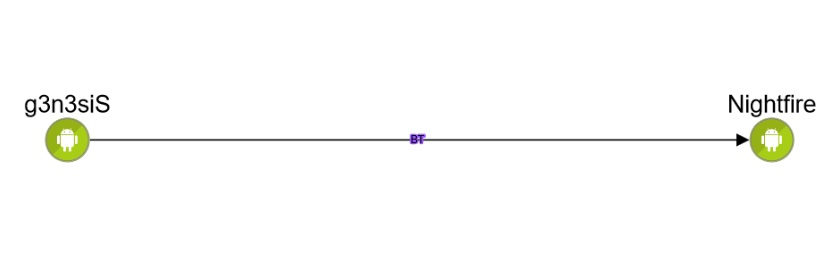
\includegraphics[width=1.0\textwidth]{belege/grosstests/Bilder/Grosstest2/Test2Misserfolg2.jpg}

2. G3n3siS verschickt eine Nachricht, die jedoch von seinem Nachbarn
Nightfire nicht weitergeleitet wird.

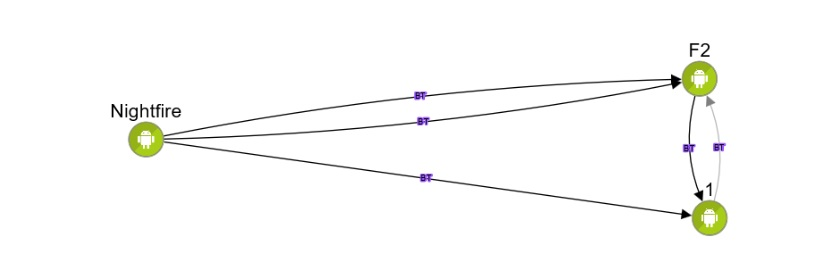
\includegraphics[width=1.0\textwidth]{belege/grosstests/Bilder/Grosstest2/Test2Misserfolg3.jpg}

3. Nightfire baut eine Verbindung zu mehreren Nachbargeräten auf, die sich
jedoch nur gegenseitig finden.

\paragraph{Schlussfolgerung aus dem Test:}

Die Anzahl der erfolgreichen Verbindungen ist sehr stark von der
funktionierenden Verbindung zwischen mnex und Sven beeinflusst.

Die Tatsache, dass extrem viele Geräte überhaupt keine Verbindung mehr
aufbauen konnten, unterstützt die Aussage, die bereits nach Test 1
getroffen wurde, dass die Limitierung der Slots nicht zielführend war.


\subsubsection{Ergebnisse Test 3}

Da wir gemerkt haben, dass die Limitierung der Slots auf 3 nicht
zielführend war, haben wir diese für Test 3 wieder rückgängig gemacht.

Wir haben auf 164 Nachrichten 11 erfolgreiche Fälle und 153 Errors.

\paragraph{Folgende Beispiele veranschaulichen Nachrichten, die beim Empfänger angekommen sind:}

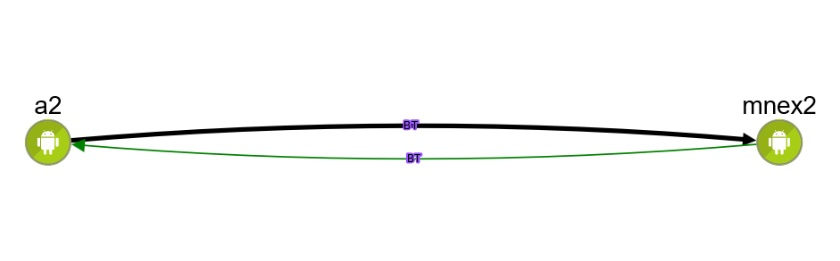
\includegraphics[width=1.0\textwidth]{belege/grosstests/Bilder/Grosstest2/Test3Erfolg1.jpg}

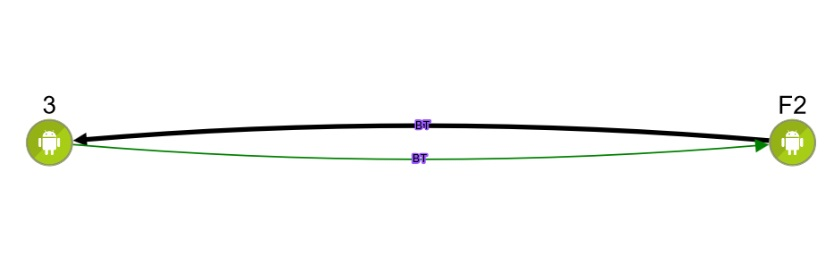
\includegraphics[width=1.0\textwidth]{belege/grosstests/Bilder/Grosstest2/Test3Erfolg2.jpg}

1 und 2. Nachrichten die zu einem benachbarten Empfänger gesendet werden.

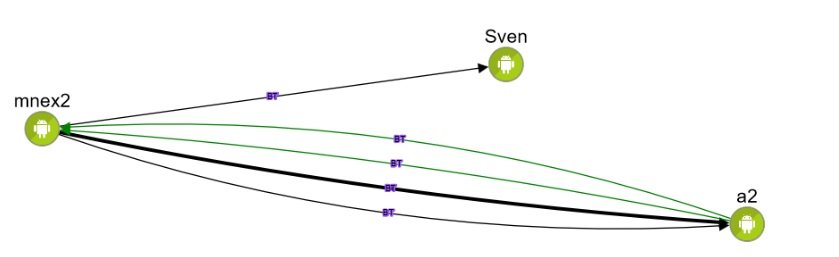
\includegraphics[width=1.0\textwidth]{belege/grosstests/Bilder/Grosstest2/Test3Erfolg3.jpg}

3. Mnex sendet eine Nachricht an Sven diese kommt jedoch erst nach dem
zweiten Versuch an. Auch das Acknowledgement benötigt zwei Versuche.

\paragraph{Folgende Beispiele veranschaulichen Nachrichten, die nicht beim Empfänger angekommen sind:}

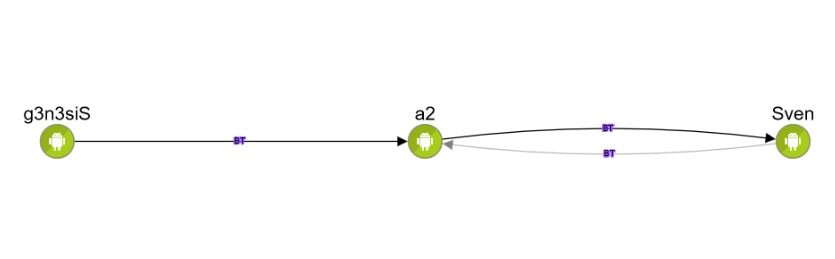
\includegraphics[width=1.0\textwidth]{belege/grosstests/Bilder/Grosstest2/Test3Misserfolg1.jpg}

1. G3n3siS sendet eine Nachricht. Diese geht jedoch nach zwei Hops verloren.\\

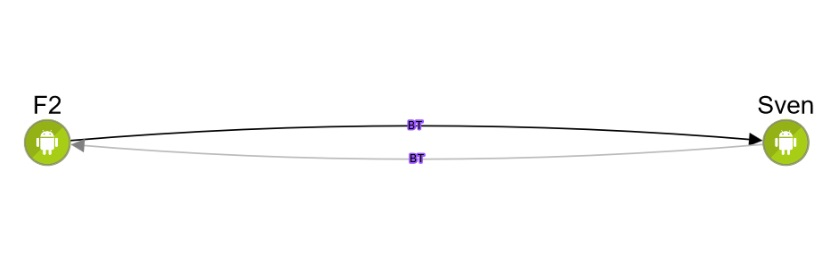
\includegraphics[width=1.0\textwidth]{belege/grosstests/Bilder/Grosstest2/Test3Misserfolg2.jpg}

2. Das wohl häufigste Beispiel des dritten Tests. Zwei benachbarte Geräte
schaffen es, eine Verbindung aufzubauen. Das zweite Handy schafft es
jedoch dann nicht, die Nachricht weiterzuleiten.


\includegraphics[width=1.0\textwidth]{belege/grosstests/Bilder/Grosstest2/Test3Misserfolg3.jpg}

3. Auch hier gab es Fälle, in denen ein Handy keine Verbindung mit einem anderen Gerät aufbauen konnte. Dies passiert jedoch deutlich seltener als bei Test 1 und 2.

\paragraph{Schlussfolgerung aus dem Test:}

Der dritte Test ist besser gelaufen als der 2. Da die Entfernung einen
erschwerenden Faktor darstellt, kann davon ausgegangen werden, dass die
Verbesserung dadurch zustande kam, dass wir die Slots nicht mehr
limitieren.

\subsubsection{Ausblick und zukünftige Tests}

Im Auftraggebertreffen wurde entschieden, dass keine weiteren
Verbesserungen am Bluetooth-Code durchgeführt werden sollen. Die Begründung
hierfür ist, dass die Implementierung des Bluetooth Stacks wohl
teilweise fehlerhaft ist.

Die Lösung hierfür ist eine eigene Implementierung des Bluetooth Stacks.
Diese soll jedoch im Rahmen einer Bachelorarbeit geschrieben werden, da
dies nicht Bestandteil des Bachelorpraktikums ist.

Da sich deshalb in der Funktionalität der Nachrichtenübertragung nichts
mehr ändern wird, haben wir auf einen dritten Großtest verzichtet.
